\documentclass[12pt,]{article}
\usepackage[left=1in,top=1in,right=1in,bottom=1in]{geometry}
\newcommand*{\authorfont}{\fontfamily{phv}\selectfont}
\usepackage[]{mathpazo}


  \usepackage[T1]{fontenc}
  \usepackage[utf8]{inputenc}




\usepackage{abstract}
\renewcommand{\abstractname}{}    % clear the title
\renewcommand{\absnamepos}{empty} % originally center

\renewenvironment{abstract}
 {{%
    \setlength{\leftmargin}{0mm}
    \setlength{\rightmargin}{\leftmargin}%
  }%
  \relax}
 {\endlist}

\makeatletter
\def\@maketitle{%
  \newpage
%  \null
%  \vskip 2em%
%  \begin{center}%
  \let \footnote \thanks
    {\fontsize{18}{20}\selectfont\raggedright  \setlength{\parindent}{0pt} \@title \par}%
}
%\fi
\makeatother




\setcounter{secnumdepth}{0}

\usepackage{longtable,booktabs}

\usepackage{graphicx,grffile}
\makeatletter
\def\maxwidth{\ifdim\Gin@nat@width>\linewidth\linewidth\else\Gin@nat@width\fi}
\def\maxheight{\ifdim\Gin@nat@height>\textheight\textheight\else\Gin@nat@height\fi}
\makeatother
% Scale images if necessary, so that they will not overflow the page
% margins by default, and it is still possible to overwrite the defaults
% using explicit options in \includegraphics[width, height, ...]{}
\setkeys{Gin}{width=\maxwidth,height=\maxheight,keepaspectratio}


\title{Political Donor Motivations and Social Media: A Time Series Analysis  }



\author{\Large \vspace{0.05in} \newline\normalsize\emph{}  }


\date{}

\usepackage{titlesec}

\titleformat*{\section}{\normalsize\bfseries}
\titleformat*{\subsection}{\normalsize\itshape}
\titleformat*{\subsubsection}{\normalsize\itshape}
\titleformat*{\paragraph}{\normalsize\itshape}
\titleformat*{\subparagraph}{\normalsize\itshape}





\newtheorem{hypothesis}{Hypothesis}
\usepackage{setspace}


% set default figure placement to htbp
\makeatletter
\def\fps@figure{htbp}
\makeatother

\usepackage{graphicx}

% move the hyperref stuff down here, after header-includes, to allow for - \usepackage{hyperref}

\makeatletter
\@ifpackageloaded{hyperref}{}{%
\ifxetex
  \PassOptionsToPackage{hyphens}{url}\usepackage[setpagesize=false, % page size defined by xetex
              unicode=false, % unicode breaks when used with xetex
              xetex]{hyperref}
\else
  \PassOptionsToPackage{hyphens}{url}\usepackage[draft,unicode=true]{hyperref}
\fi
}

\@ifpackageloaded{color}{
    \PassOptionsToPackage{usenames,dvipsnames}{color}
}{%
    \usepackage[usenames,dvipsnames]{color}
}
\makeatother
\hypersetup{breaklinks=true,
            bookmarks=true,
            pdfauthor={ ()},
             pdfkeywords = {},  
            pdftitle={Political Donor Motivations and Social Media: A Time Series Analysis},
            colorlinks=true,
            citecolor=blue,
            urlcolor=blue,
            linkcolor=magenta,
            pdfborder={0 0 0}}
\urlstyle{same}  % don't use monospace font for urls

% Add an option for endnotes. -----


% add tightlist ----------
\providecommand{\tightlist}{%
\setlength{\itemsep}{0pt}\setlength{\parskip}{0pt}}

% add some other packages ----------

% \usepackage{multicol}
% This should regulate where figures float
% See: https://tex.stackexchange.com/questions/2275/keeping-tables-figures-close-to-where-they-are-mentioned
\usepackage[section]{placeins}


\begin{document}
	
% \pagenumbering{arabic}% resets `page` counter to 1 
%
% \maketitle

{% \usefont{T1}{pnc}{m}{n}
\setlength{\parindent}{0pt}
\thispagestyle{plain}
{\fontsize{18}{20}\selectfont\raggedright 
\maketitle  % title \par  

}

{
   \vskip 13.5pt\relax \normalsize\fontsize{11}{12} 
\textbf{\authorfont } \hskip 15pt \emph{\small }   

}

}






\vskip -8.5pt


 % removetitleabstract

\noindent \doublespacing 

The two predominant theories of political donor motivations are the
access-oriented model and the consumption model. This paper combines
political donation records and social media posts from politicians to
test whether either behavior is observed. In the access-oriented model,
individual political donors and political action committees (PACs) are
assumed to contribute to campaigns in an effort to acquire access and
influence politicians into supporting specific policy issues. In this
study, the access-oriented model of donors predicts that donations from
specific groups of donors will precede public support of certain
policies. The consumption model of donors views political contributions
as being an extension of voting along a participatory spectrum, and that
donors support candidates who they already know support policy issues
that the donors care about or are ideologically motivated. In this
research, the consumption model predicts that donations from various
groups of donors will lag in response to public support of certain
policy issues. Historically, these two models have treated political
donors as all having the same motivations. More recent studies in
campaign finance have found that both motivational models can exist in
different groups of donors. However, these studies categorize groups of
donors in broad strokes, generally as either small-dollar donors and
large-dollar donors as well as PACs. This paper statistically derives
coalitions of similar donors and tests the competing models of political
donor motivations on these more granular groups of donors who support
similar candidates.

\begin{longtable}[]{@{}lll@{}}
\toprule
Method & koRpus & stringi\tabularnewline
\midrule
\endhead
Word count & 1676 & 1679\tabularnewline
Character count & 11389 & 11388\tabularnewline
Sentence count & 70 & Not available\tabularnewline
Reading time & 8.4 minutes & 8.4 minutes\tabularnewline
\bottomrule
\end{longtable}

\hypertarget{introduction}{%
\section{Introduction}\label{introduction}}

{[}Need some sort of bridge into specific models{]}

\hypertarget{access-oriented-model}{%
\section{Access-Oriented Model}\label{access-oriented-model}}

Access-oriented political donors are those that attempt to use their
contributions to gain access to politicians. Most often, access-oriented
donors are thought to be the motivation behind contributions from
Political Action Committees (PACs) and donors with business interest.
The theory goes that this access can then influence legislative behavior
(Francia et al. 2003). Milbrath (1958) centers legislative influence as
a communicative process where those seeking to influence legislators
must be able to ``communicate their power, as well as the facts and
arguments supporting their position, when they confer with a
legislator.'' Congress is operating in a ``vacuum filled with noise.''
And political contributions can gain direct access that allows to to cut
through all the noise of competing information that the legislator might
be encountering (Milbrath 1958). In interviews, business groups
themselves said that they seek ``access'' to either a member of congress
or a member of their staff when they make a contribution. But these
groups stated that their contribution only gains the access to make an
argument and it is the merit of the argument that determines support for
their cause or not (Herndon 1982). Empirical studies of financial
documents backup this claim that donors seek access in order to
influence policy (Fouirnaies and Hall 2015). Past research has suggested
that political contributors are successful in their goals to gain access
as measured by the amount of time that organized interest groups spend
with members of congress (Langbein 1986).

However, measuring the direct access that political financiers gain from
political contributions is difficult to measure. Instead, researchers
have treated the ``access'' component of contributor influence as an
implicit assumption and instead look for evidence of ``influence'' of
political contributors on politicians. Many political science papers do
not use the explicit term ``access-oriented donor'' and instead refer to
their work as examining the potential ``influence'' of political donors
on politicians. This line of influence research implies a gain of access
by political contributors. As Langbein (1986) states, ``{[}Access{]} is
a precondition for having influence over public policy. Contributions
themselves have little meaning for a congressman, because they do not
carry any `message.' Only access, or some other form of direct or
indirect communication, can translate money into influence.''

Even though research has suggested there is a connection between
political contributions and access. It is unclear if that access
actually converts to \emph{influence} in the political process. Despite
confirmation that PACs attempt to influence the legislative process
(Grenzke 1989), past research has found PAC contributions to have a
limited effect on roll-call voting (Wright 1985). In rare instances,
there is an apparent connection between PAC contributions and roll-call
votes, but it that correlation is most likely due to broader support
from larger interest groups (Grenzke 1989). These sparse correlations
could be manifestation of the finding that legislators are responsive to
changes to the opinions of the national individual donor class
(Canes-Wrone and Gibson 2019). One article went so far as to conclude
that ``evidence in the article undermines belief in the
military-industrial complex model'' (Wayman 1985) when studying the
effect of defense-related PACs on roll-call voting.

Other studies on the connection between campaign contributions and
legislative voting does support that moneyed interests play a
significant role in the legislative process, particularly organized
business interests that are within a member's district (Hall and Wayman
1990), potentially similar to how members of congress prioritize public
opinion of their district over national public opinion {[}butler2011{]}.
Further, there appears to be a stronger influence as a result of
contributions from individuals with business interests, opposed to PACs,
which many other studies focus on (Fellowes and Wolf 2004). A
meta-analysis found that model specification played a significant role
in whether significant results were found when looking for a connection
between donations and roll-calls votes, concluding that studies that
controlled for ``friendly giving by including a measure of legislators'
ideology and that include more than one contributions variable are less
likely to produce significant results'' (Roscoe and Jenkins 2005).
Despite this variability in model specification, the authors conclude
that one-third of roll-call votes are impacted by campaign contributions
(Roscoe and Jenkins 2005).

Potentially, the influence exerted by contributors when making a
political contribution is so indirect that it doesn't always materialize
in statistical patterns of legislative voting, but there is evidence of
the influence as a result of the legislation. For example, one study
found that future returns of firms is positively and significantly
correlated with contributions in support for candidates, finding the
strongest effect among firms that support candidates within the state
that the firm is based (Cooper, Gulen, and Ovtchinnikov 2010). In
addition to immediately-felt financial returns, donors may
systematically contribute money to legislative agenda setters, such as
chairs of financial committees, in an effort to set future legislative
agendas (Fouirnaies 2018). Even campaign contribution from business
executives are ``best understood as purchases of `good will' whose
returns, while positive in expectation, are contingent and rare''
(Gordon, Hafer, and Landa 2007).

\hypertarget{consumption-model}{%
\section{Consumption Model}\label{consumption-model}}

\hypertarget{online-fundraising}{%
\section{Online Fundraising}\label{online-fundraising}}

\hypertarget{rise-of-small-dollar-donors}{%
\section{Rise of Small-Dollar
Donors}\label{rise-of-small-dollar-donors}}

\hypertarget{ideological-measurement-using-donor-data}{%
\section{Ideological Measurement Using Donor
Data}\label{ideological-measurement-using-donor-data}}

\hypertarget{data}{%
\section{Data}\label{data}}

Data for this research comes from two primary sources: politicians'
social media posts and political donation data. For social media posts,
this paper used the Facebook (Barbera, Geisler, and Atteveldt 2017) and
Twitter (Kearney 2019) APIs to collect social media posts from all
candidates for the Wisconsin State Senate and Wisconsin State Assembly
during the 2016 election cycle (\emph{n} = 82,851). A subset of these
posts were hand-coded into 27 topical categories. This subset was used
to train a BERT deep learning transfer model that was used to predict
the topic of the remainder of the posts (training dataset = 8,242, 10\%
of total posts; testing dataset = 4,122, 5\% of total posts). Political
donation data for all candidates to the Wisconsin State Legislature
during the 2016 election cycle were collected from the Wisconsin
Campaign Information System (CFIS) (\emph{n} = 12,962). These donations
were used to create a network of political donations with candidates and
donors serving as nodes and donations between them as edges. This
network was clustered into distinct communities so that donors in each
community are most similar to one another based on which campaigns they
contributed to. I theorize that these clusters of donors represent
\emph{latent coalitions} of donors who, whether they operate in an
organized fashion or not, are working toward the goal of electing the
same candidates. Studying political fundraisers as members of political
coalitions has been studied in the past (Adams 2007; Heerwig 2016). This
paper's statistically-driven definition of latent coalitions seeks to
add to the coalition literature.

\hypertarget{methodology}{%
\section{Methodology}\label{methodology}}

These two datasets were analyzed against each other using the Granger
causality time-series methodology. This methodology has been used by
other researchers to study social media (Freelon, McIlwain, and Clark
2018; Lukito 2020). Similar to political donations, this methodology has
been used to study the relationship between social media and non-social
media events such as offline protests (Bastos, Mercea, and Charpentier
2015) and stock prices (Park, Leung, and Ma 2017). Granger causality
detects whether movements in one time series precedes, lags, has a
confounding variable, or is not related to another time series.
Specifically, this paper compares time series of donations from clusters
of political donors and time series of the number of social media posts
by each topic that were made by campaigns that each donor cluster
contributed to. For example, a time series of donations from a donor
coalition was compared to the aggregate count of posts about a given
topic made by candidates that the donor cluster contributed to.

\hypertarget{preliminary-results}{%
\section{Preliminary Results}\label{preliminary-results}}

Initial results suggest that it is more common to observe behavior
consistent with the consumption model (31\% of coalitions, 4/13) than
the access-oriented model. However, the access-oriented model is still
observed in 15\% of coalitions (2/13). Under a strict interpretation of
either model, we would expect to find behavior that fits only with that
model. These results that find both the models present in the data is in
line with some other research in suggesting that there are a ``diversity
of roles individual contributors play in the campaign finance system''
(Heerwig 2016). Specific results of the Granger causality model are in
Figure 1 below.

\begin{figure}
\centering
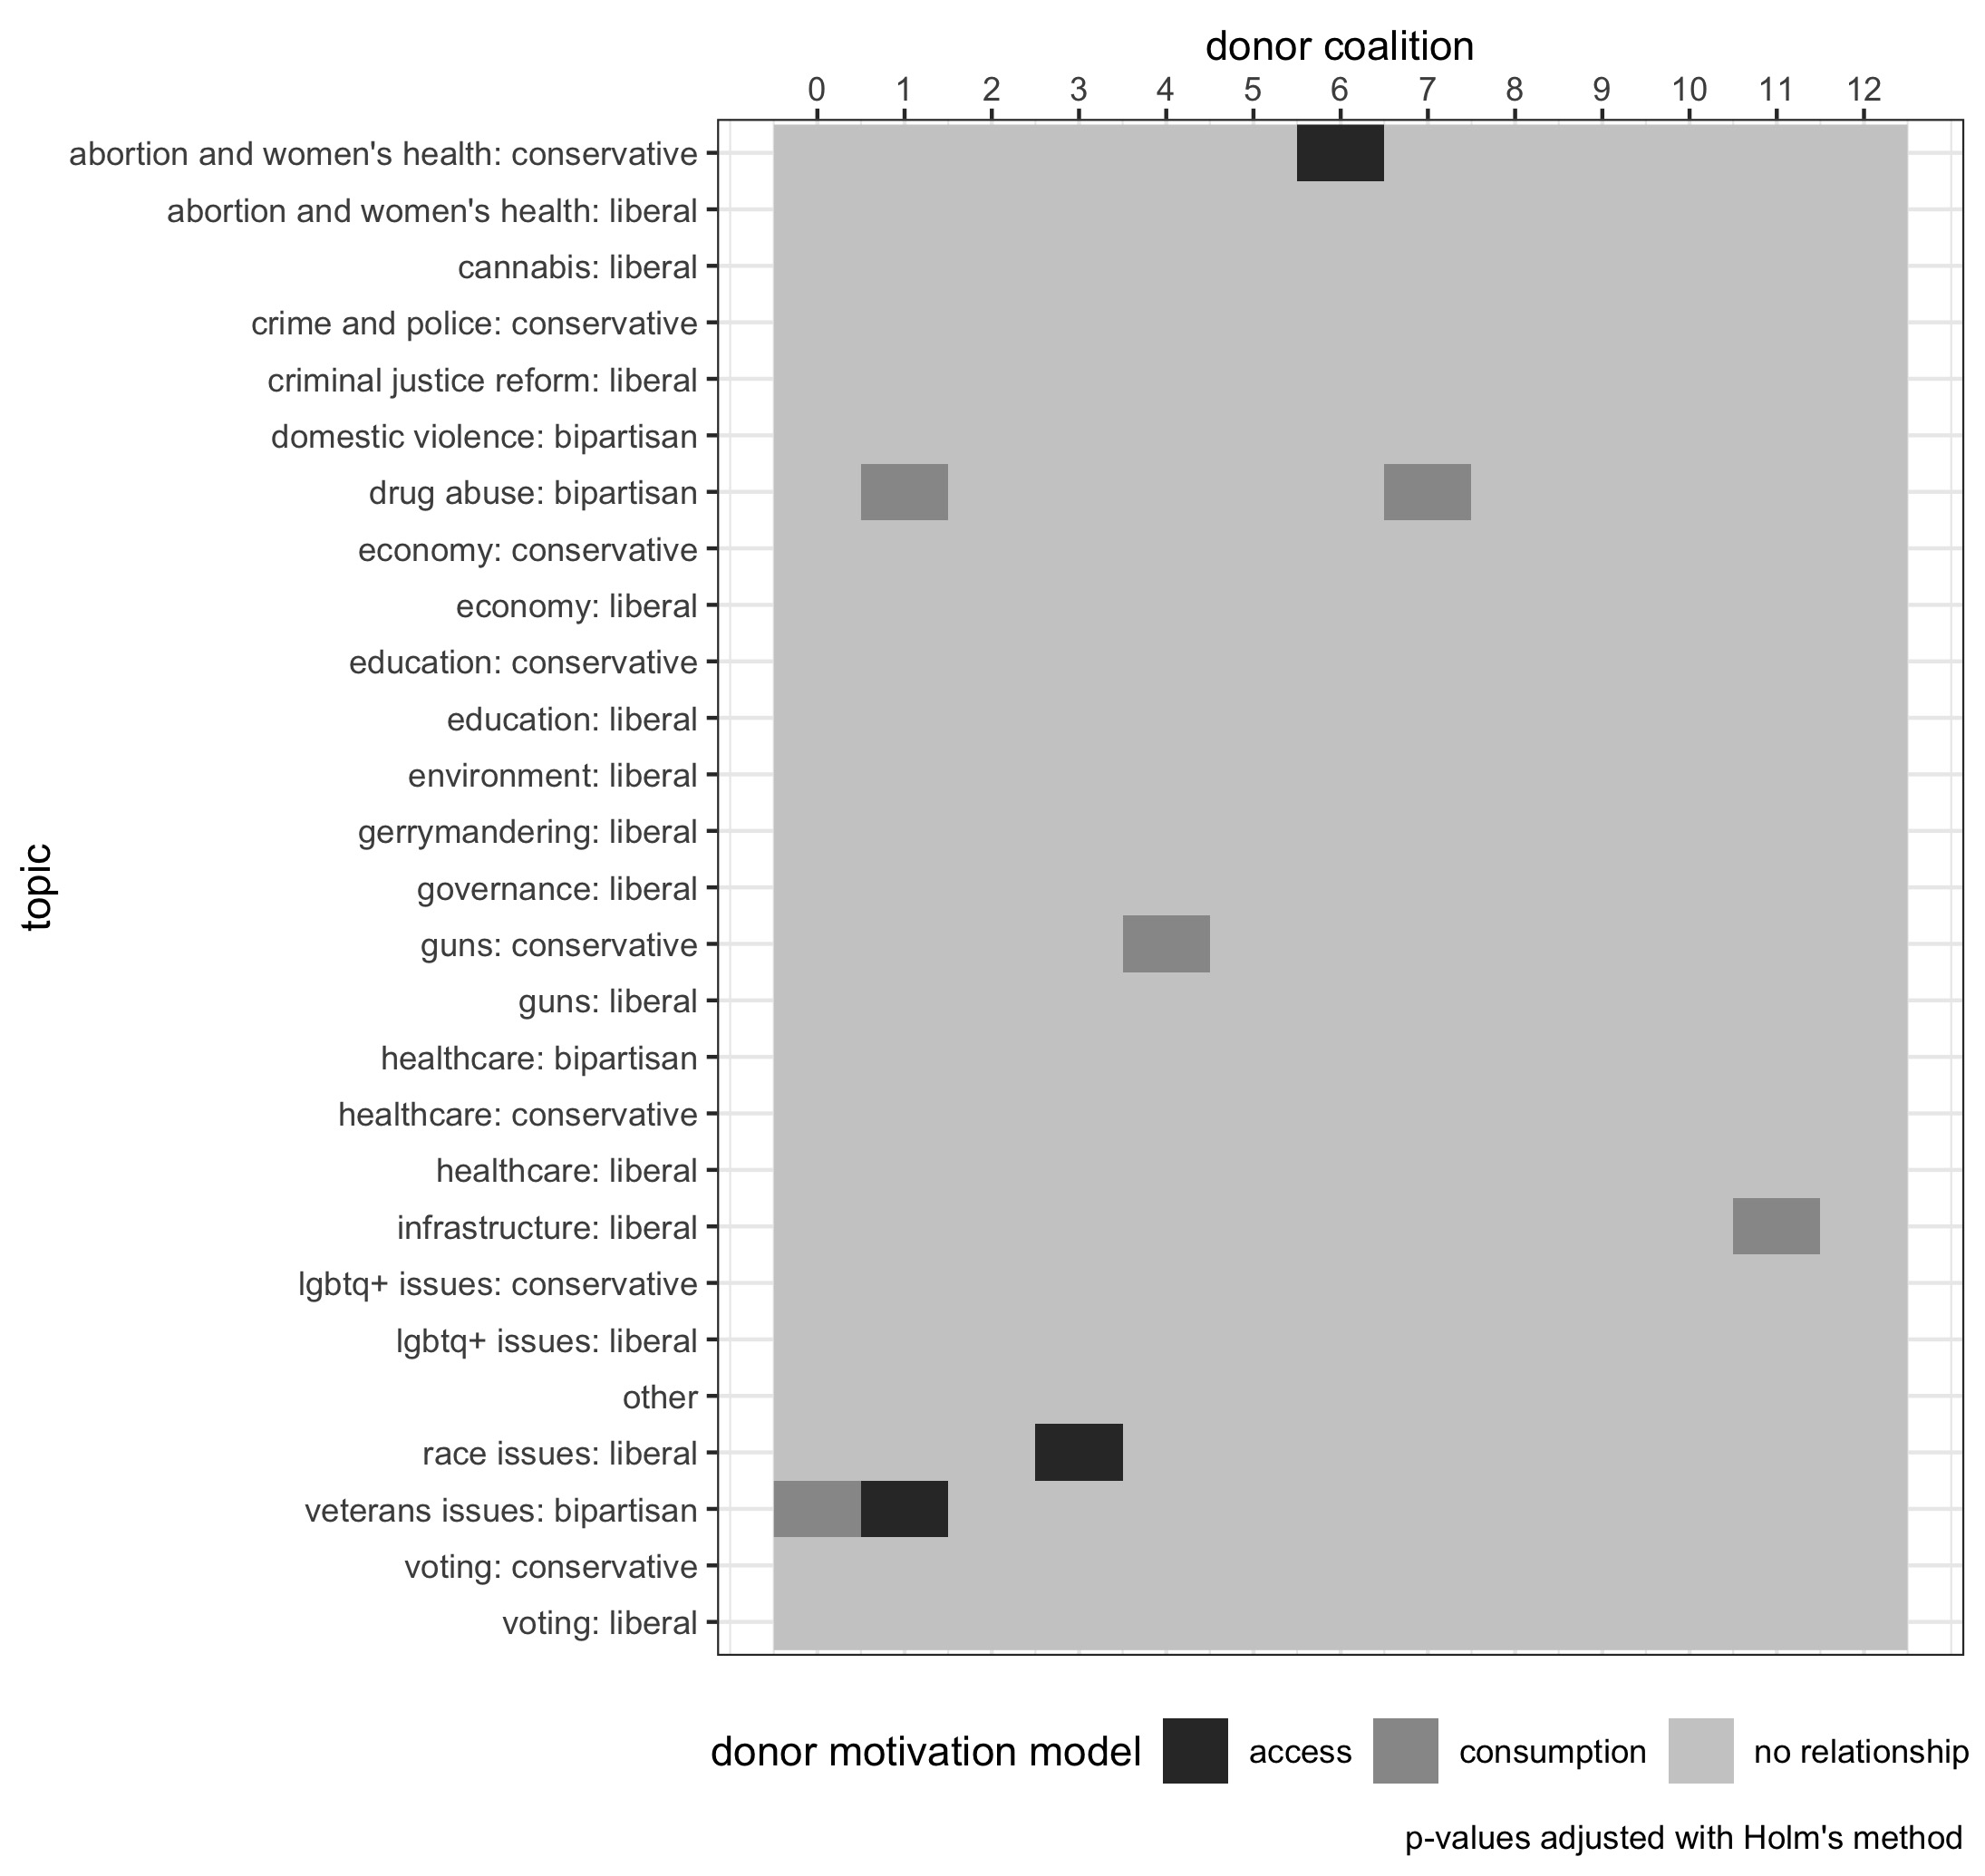
\includegraphics{../tables_and_figures/aejmc_abstract_1.jpg}
\caption{Donor Motivation Models}
\end{figure}

One theoretical next step for this paper is to flesh out the
implications of observing behavior that fits under both the consumption
and access-oriented model of political donors. Most often, the
literature assumes that political donors have monolithic a monolithic
psychological process that motivate them. However, the clear breakdown
of different coalitions exhibiting behavior that falls into different
models, and distinct behavior in relation to unique policy issues,
suggests that latent coalitions of political donors are strategic actors
with unique motivations. One empirical next step is to quantify
potential confounders for donor clusters that don't fit under either
model, such as geographic proximity or competitiveness of the races
contributed to.

\hypertarget{references}{%
\section*{References}\label{references}}
\addcontentsline{toc}{section}{References}

\hypertarget{refs}{}
\leavevmode\hypertarget{ref-adams2016}{}%
Adams, Brian E. 2007. ``Fundraising Coalitions in Open Seat Mayoral
Elections.'' \emph{Journal of Urban Affairs} 29 (5): 481--99.
\url{https://doi.org/10.1111/j.1467-9906.2007.00361.x}.

\leavevmode\hypertarget{ref-rfacebook}{}%
Barbera, Pablo, Andrew Geisler, and Wouter van Atteveldt. 2017.
\emph{Rfacebook}.
\url{https://cran.r-project.org/web/packages/Rfacebook/Rfacebook.pdf}.

\leavevmode\hypertarget{ref-bastos2015}{}%
Bastos, Marco T., Dan Mercea, and Arthur Charpentier. 2015. ``Tents,
Tweets, and Events: The Interplay Between Ongoing Protests and Social
Media.'' \emph{Journal of Communication} 65 (2): 320--50.
\url{https://doi.org/10.1111/jcom.12145}.

\leavevmode\hypertarget{ref-caneswrone2019}{}%
Canes-Wrone, Brandice, and Nathan Gibson. 2019. ``Does Money Buy
Congressional Love? Individual Donors and Legislative Voting.''
\emph{Congress \& the Presidency} 46 (1): 1--27.
\url{https://doi.org/10.1080/07343469.2018.1518965}.

\leavevmode\hypertarget{ref-cooper2010}{}%
Cooper, Michael J., Huseyin Gulen, and Alexei V. Ovtchinnikov. 2010.
``Corporate Political Contributions and Stock Returns.'' \emph{The
Journal of Finance} 65 (2): 687--724.
\url{https://doi.org/https://doi.org/10.1111/j.1540-6261.2009.01548.x}.

\leavevmode\hypertarget{ref-fellowes2004}{}%
Fellowes, Matthew C., and Patrick J. Wolf. 2004. ``Funding Mechanisms
and Policy Instruments: How Business Campaign Contributions Influence
Congressional Votes.'' \emph{Political Research Quarterly} 57 (2):
315--24.

\leavevmode\hypertarget{ref-fouirnaies2018}{}%
Fouirnaies, Alexander. 2018. ``When Are Agenda Setters Valuable?''
\emph{American Journal of Political Science} 62 (1): 176--91.
\url{https://doi.org/https://doi.org/10.1111/ajps.12316}.

\leavevmode\hypertarget{ref-fouirnaies2015}{}%
Fouirnaies, Alexander, and Andrew Hall. 2015. ``The Exposure Theory of
Access: Why Some Firms Seek More Access to Incumbents Than Others.''
\emph{SSRN Electronic Journal}, January.
\url{https://doi.org/10.2139/ssrn.2652361}.

\leavevmode\hypertarget{ref-francia2003}{}%
Francia, Peter L., John C. Green, Paul S. Herrnson, Lynda W. Powell, and
and Clyde Wilcox. 2003. \emph{The Financiers of Congressional
Elections}. New York, NY: Columbia University Press.

\leavevmode\hypertarget{ref-freelon2018}{}%
Freelon, D, C McIlwain, and M Clark. 2018. ``Quantifying the Power and
Consequences of Social Media Protest.'' \emph{New Media \& Society} 20
(3): 990--1011. \url{https://doi.org/10.1177/1461444816676646}.

\leavevmode\hypertarget{ref-gordon2007}{}%
Gordon, Sanford C., Catherine Hafer, and Dimitri Landa. 2007.
``Consumption or Investment? On Motivations for Political Giving.''
\emph{The Journal of Politics} 69 (4): 1057--72.

\leavevmode\hypertarget{ref-grenzke1989}{}%
Grenzke, Janet M. 1989. ``PACs and the Congressional Supermarket: The
Currency Is Complex.'' \emph{American Journal of Political Science} 33
(1): 1--24. \url{http://www.jstor.org/stable/2111251}.

\leavevmode\hypertarget{ref-hall1990}{}%
Hall, Richard L., and Frank W. Wayman. 1990. ``Buying Time: Moneyed
Interests and the Mobilization of Bias in Congressional Committees.''
\emph{American Political Science Review} 84 (3): 797--820.
\url{https://doi.org/10.2307/1962767}.

\leavevmode\hypertarget{ref-heerwig2016}{}%
Heerwig, Jennifer A. 2016. ``Donations and Dependence: Individual
Contributor Strategies in House Elections.'' \emph{Social Science
Research} 60: 181--98.
\url{https://doi.org/https://doi.org/10.1016/j.ssresearch.2016.06.001}.

\leavevmode\hypertarget{ref-herndon1982}{}%
Herndon, James F. 1982. ``Access, Record, and Competition as Influences
on Interest Group Contributions to Congressional Campaigns.'' \emph{The
Journal of Politics} 44 (4): 996--1019.

\leavevmode\hypertarget{ref-rtweet}{}%
Kearney, Michael W. 2019. ``Rtweet: Collecting and Analyzing Twitter
Data.'' \emph{Journal of Open Source Software} 4 (42): 1829.
\url{https://doi.org/10.21105/joss.01829}.

\leavevmode\hypertarget{ref-langbein1986}{}%
Langbein, Laura I. 1986. ``Money and Access: Some Empirical Evidence.''
\emph{The Journal of Politics} 40 (4): 1052--62.

\leavevmode\hypertarget{ref-lukito2020}{}%
Lukito, Josephine. 2020. ``Coordinating a Multi-Platform Disinformation
Campaign: Internet Research Agency Activity on Three U.s. Social Media
Platforms, 2015 to 2017.'' \emph{Political Communication} 37 (2):
238--55. \url{https://doi.org/10.1080/10584609.2019.1661889}.

\leavevmode\hypertarget{ref-milbrath1958}{}%
Milbrath, Lester W. 1958. ``The Political Party Activity of Washington
Lobbyists.'' \emph{The Journal of Politics} 20 (2): 339--52.

\leavevmode\hypertarget{ref-park2017}{}%
Park, J., H. Leung, and K. Ma. 2017. ``Information Fusion of Stock
Prices and Sentiment in Social Media Using Granger Causality.'' In
\emph{2017 Ieee International Conference on Multisensor Fusion and
Integration for Intelligent Systems (Mfi)}, 614--19.
\url{https://doi.org/10.1109/MFI.2017.8170390}.

\leavevmode\hypertarget{ref-roscoe2005}{}%
Roscoe, Douglas D., and Shannon Jenkins. 2005. ``A Meta-Analysis of
Campaign Contributions' Impact on Roll Call Voting*.'' \emph{Social
Science Quarterly} 86 (1): 52--68.
\url{https://doi.org/https://doi.org/10.1111/j.0038-4941.2005.00290.x}.

\leavevmode\hypertarget{ref-wayman1985}{}%
Wayman, Frank Whelon. 1985. ``Arms Control and Strategic Arms Voting in
the U.s. Senate: Patterns of Change, 1967-1983.'' \emph{The Journal of
Conflict Resolution} 29 (2): 225--51.
\url{http://www.jstor.org/stable/174100}.

\leavevmode\hypertarget{ref-wright1985}{}%
Wright, John R. 1985. ``PACs, Contributions, and Roll Calls: An
Organizational Perspective.'' \emph{American Political Science Review}
79 (2): 400--414. \url{https://doi.org/10.2307/1956656}.





\newpage
\singlespacing 
\end{document}
